%%%%%%%%%%%%%%%%%%%%%%%%%%%%%%%%%%%%%%%%%%%%%%%%%%%%%%%%
%%%%%%%%%------RMIT SPACE POSTER------------%%%%%%%%%%%%
%%%%%%%%%%%%%%%%%%%%%%%%%%%%%%%%%%%%%%%%%%%%%%%%%%%%%%%%
%%%%%%%%%%%%%%%%%%%%%%%%%%%%%%%%%%%%%%%%%%%%%%%%%%%%%%%%
% a0poster Portrait Poster
%
% The a0poster class was created by:
% Gerlinde Kettl and Matthias Weiser (tex@kettl.de)
% 
% License:
% CC BY-NC-SA 3.0 (http://creativecommons.org/licenses/by-nc-sa/3.0/)
%
% Author/Designer: Timothy Kodikara
%
%% Note: CRC and SERC logos are included in the /figures folder if you might want to use them.
%%%%%%%%%%%%%%%%%%%%%%%%%%%%%%%%%%%%%%%%%
%----------------------------------------------------------------------------------------
%	PACKAGES AND OTHER DOCUMENT CONFIGURATIONS
%----------------------------------------------------------------------------------------
\documentclass[a0,portrait]{a0poster}
%%
\usepackage[top=5cm, bottom=0.3cm, left=5cm, right=3cm]{geometry}
\usepackage[compact]{titlesec}
\usepackage{multicol} % This is so we can have multiple columns of text side-by-side
\columnsep=100pt % This is the amount of white space between the columns in the poster
\columnseprule=10pt % This is the thickness of the blue line between the columns in the poster
\usepackage[svgnames]{xcolor} % Specify colors by their 'svgnames', for a full list of all colors available see here: http://www.latextemplates.com/svgnames-colors
%\usepackage{times} % Use the times font
\usepackage{palatino} % Uncomment to use the Palatino font
\usepackage{xkeyval}
\usepackage{graphicx} % Required for including images
\setlength{\abovecaptionskip}{5pt plus 5pt minus 3pt}
\graphicspath{{figures/}} % Location of the graphics files
\usepackage{booktabs} % Top and bottom rules for table
\usepackage[font=small,labelfont=bf]{caption} % Required for specifying captions to tables and figures
\usepackage{amsfonts, amsmath, amsthm, amssymb} % For math fonts, symbols and environments
\usepackage{csquotes}
\usepackage{wrapfig} % Allows wrapping text around tables and figures
%\usepackage[pdftex]{color}
\def\columnseprulecolor{\color{Orange}}%
\usepackage{framed}
\colorlet{frameborder}{Orange}
%----------------------------------------------------------------------------------------
%	POSTER HEADER 
%----------------------------------------------------------------------------------------
% The header is divided into three boxes:
% The widths of these boxes can be easily edited to accommodate your content as you see fit
\begin{document}
%\hspace*{0.2cm}
\begin{minipage}[c]{\linewidth}
\vspace{0.1cm}
\noindent\makebox[\textwidth][c]{
\begin{minipage}[c]{0.10\linewidth}
\vspace{0pt}\raggedright
\hspace{1cm}
\includegraphics[width=1.5\linewidth]{SUSTech}
\end{minipage}
\hfill
\begin{minipage}[c]{0.70\textwidth}
\centering
\Huge \color{NavyBlue} \textbf{Automated EEG-based major depress disorder detection through transformer-based network}\\[0.5cm]
\large \color{Black} \textbf{Ziyan Zhang$^{1}$, Zhe Cao$^{1}$, Weiqi Ruan$^{1}$}\\[0.2cm] % Author(s)
\small 1. Institute for Quantum Science and Engineering, SUSTech, Shenzhen, China\\[0.1cm] % University
\small \texttt{Correspondence: 12132873@mail.sustech.edu.cn}\\
\small \texttt{12132834@mail.sustech.edu.cn}\\
\small \texttt{1023104572@qq.com}\\
\end{minipage}
%\hfill
\begin{minipage}[c]{0.15\textwidth}
\vspace{0pt}\raggedleft
\includegraphics[scale=1,width=1.1\linewidth]{BME5012}
\hspace{1cm}
\end{minipage}}
\\[0.1cm]%
% A bit of extra whitespace between the header and poster content
%----------------------------------------------------------------------------------------
\color{Orange}\setlength\FrameRule{10pt}
\begin{framed}
\vspace{0.5cm}
\begin{multicols}{2} % This is how many columns your poster will be broken into, a portrait poster is generally split into 2 columns
%----------------------------------------------------------------------------------------
%	INTRODUCTION
%----------------------------------------------------------------------------------------
\color{Black}
\section*{Introduction}
In recent years, deep learning has been extensively used for arbitrary diagnosis of many mental diseases based on EEG or fMRI, including epilepsy$^1$, seizure prediction$^2$, Alzheimer's disease$^3$, etc. Simultaneously, depression is a common illness worldwide, with an estimated 3.8\% of the population affected, including 5.0\% among adults and 5.7\% among adults older than 60 years. Over 700,000 people die due to suicide caused by the depression every year. $^4$  However, it can be effectively diagnosed and treated in early period. A schematic comparison of synapses from a healthy subject and a depressed subject is presented in Fig. 1.\\
%\begin{wrapfigure}{R}{0.25\textwidth}
\begin{center}
\hspace*{\fill}
\includegraphics[width=0.4\linewidth]{figures/normal_syn}
\includegraphics[trim={0 0.9cm 0 0},clip,width=0.49\linewidth]{figures/abnormal}
\captionof{figure}{\color{Green}A schematic comparison of synapses of a healthy subject (left) and a depressed patient (right)$^5$.}
\label{IGSMap}
\end{center}
In this work, we presented an EEG-based major depress disorder detection neural network based on transformer. It takes EEG signal as input and outputs its predication graded with None, Mild, Moderate and Severe based on the severity of symptoms. We trained this network with 128 channels resting signal obtained 24 major depressive disorder subjects and 29 healthy control subjects, ranging from 16 - 52 years old$^6$. This model was tested by various public datasets, the accuracy and f1 score can reach over 0.8. Additionally, we compared our network with naive CNN and RNN, it can be inducted that our model performs better.
%----------------------------------------------------------------------------------------
%	METHODS
%---------------------------------------------------------------------------------------- 
\color{Black}
\section*{Data and Methods}
%\begin{wrapfigure}{R}{0.25\textwidth}
%\centering
%\end{wrapfigure}
The data being used in this work is an open-source EEG dataset from UAIS Lab, Lanzhou University, China$^6$. The dataset contains traditional 128-electrodes EEG signals as well as audio data from clinically depressed patients and matching normal controls. The EEG signals of 53 subjects were recorded in resting state \& under stimulation.  \\
\begin{center}
\hspace*{\fill}
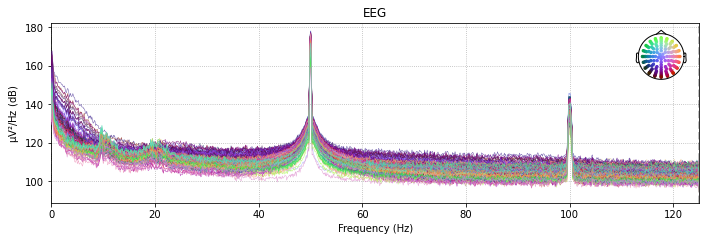
\includegraphics[width=0.49\linewidth]{figures/mdd}
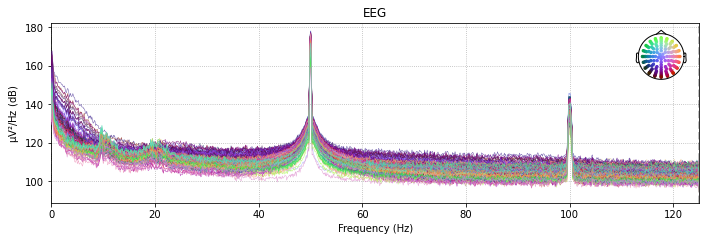
\includegraphics[clip,width=0.49\linewidth]{figures/hc}
\captionof{figure}{\color{Green}Comparison of power spectral densities of WDD(left) and HC(right).}
\label{IGSMap}
\end{center}
%\hspace{0.1cm}$\circ$ Sdfshd d: 25\textendash31 January, 2015;\\
%\hspace{0.1cm}$\circ$ Redfshdghgons (Fig.\ref{IGSMap}): Lorem ipsum dolor sit amet, consectetur adipiscing elit, sed;\\
%\hspace{0.1cm}$\circ$ Geomagnetic activity: Kp $<$ 4 throughout the study period;\\
%\hspace{0.1cm}$\circ$ Analysis: Two types of accuracy and;\\
%\hspace{0.1cm}$\circ$ GIR: Lorem ipsum dolor sit amet, consectetur adipiscing elit, sed do eiusmod tempor;\\
%\hspace{0.1cm}$\circ$ AGD: Lsunt in culpa qui officia deserunt mollit anim id est laborum.\\
The pre-processing of the raw EEG signal contains 3 parts, 
\begin{enumerate}
\item Segmenting
\item Band-pass filtering
\item Standarlization
\end{enumerate}
The data is segmented into trials as $C_{eeg}*T$, where $C_{eeg}$ is the number of EEG channels and $T$ is the sample points. Then we add band-pass filter data to $[4,40]Hz$ to remove high and low-frequency noise. After that we apply standard normalization to relive the fluctuation and non-stationarity  as $$X=\frac{{x-\mu}}{{\sqrt{\sigma}^2}}$$Additionally, we give a feasible way based on CSP usage to improve the difference of the original signal and maintain the temporal information.
\begin {center}
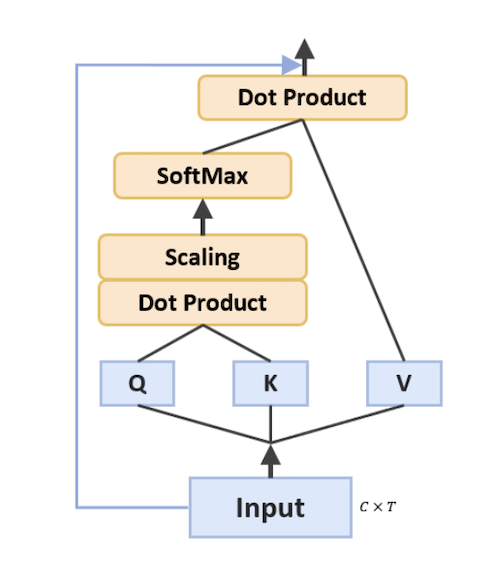
\includegraphics{figures/dot}
\captionof{figure}{\color{Green}The calculation process of spatial feature-channel attention}
\label{dot}
\end{center}
We proposed a method of feature channel weighting inspired by the scaled dot-product$^7$. As illustrated in Fig.\ref{dot}. The input data is first linearly transformed into vectors, queries($Q$), and keys($K$). The whole process can be expressed as $$Attention(Q, K, V) = \frac{QK^{T}}{d_k}V$$Additionally, we perceiving global temporal dependencies of EEG signals using the attention mechanism. In the beginning, the data is compressed to one dimension $1{\times}T$ to reduce the computational complexity, since the feature channels have been weighted in the previous step. Therefore, we divide the data into multiple slices with a shape of $1{\times}d$ for attention training. After that, we simply apply global average pooling to generate the results. We showed the whole process in Fig.4\\
\begin {center}
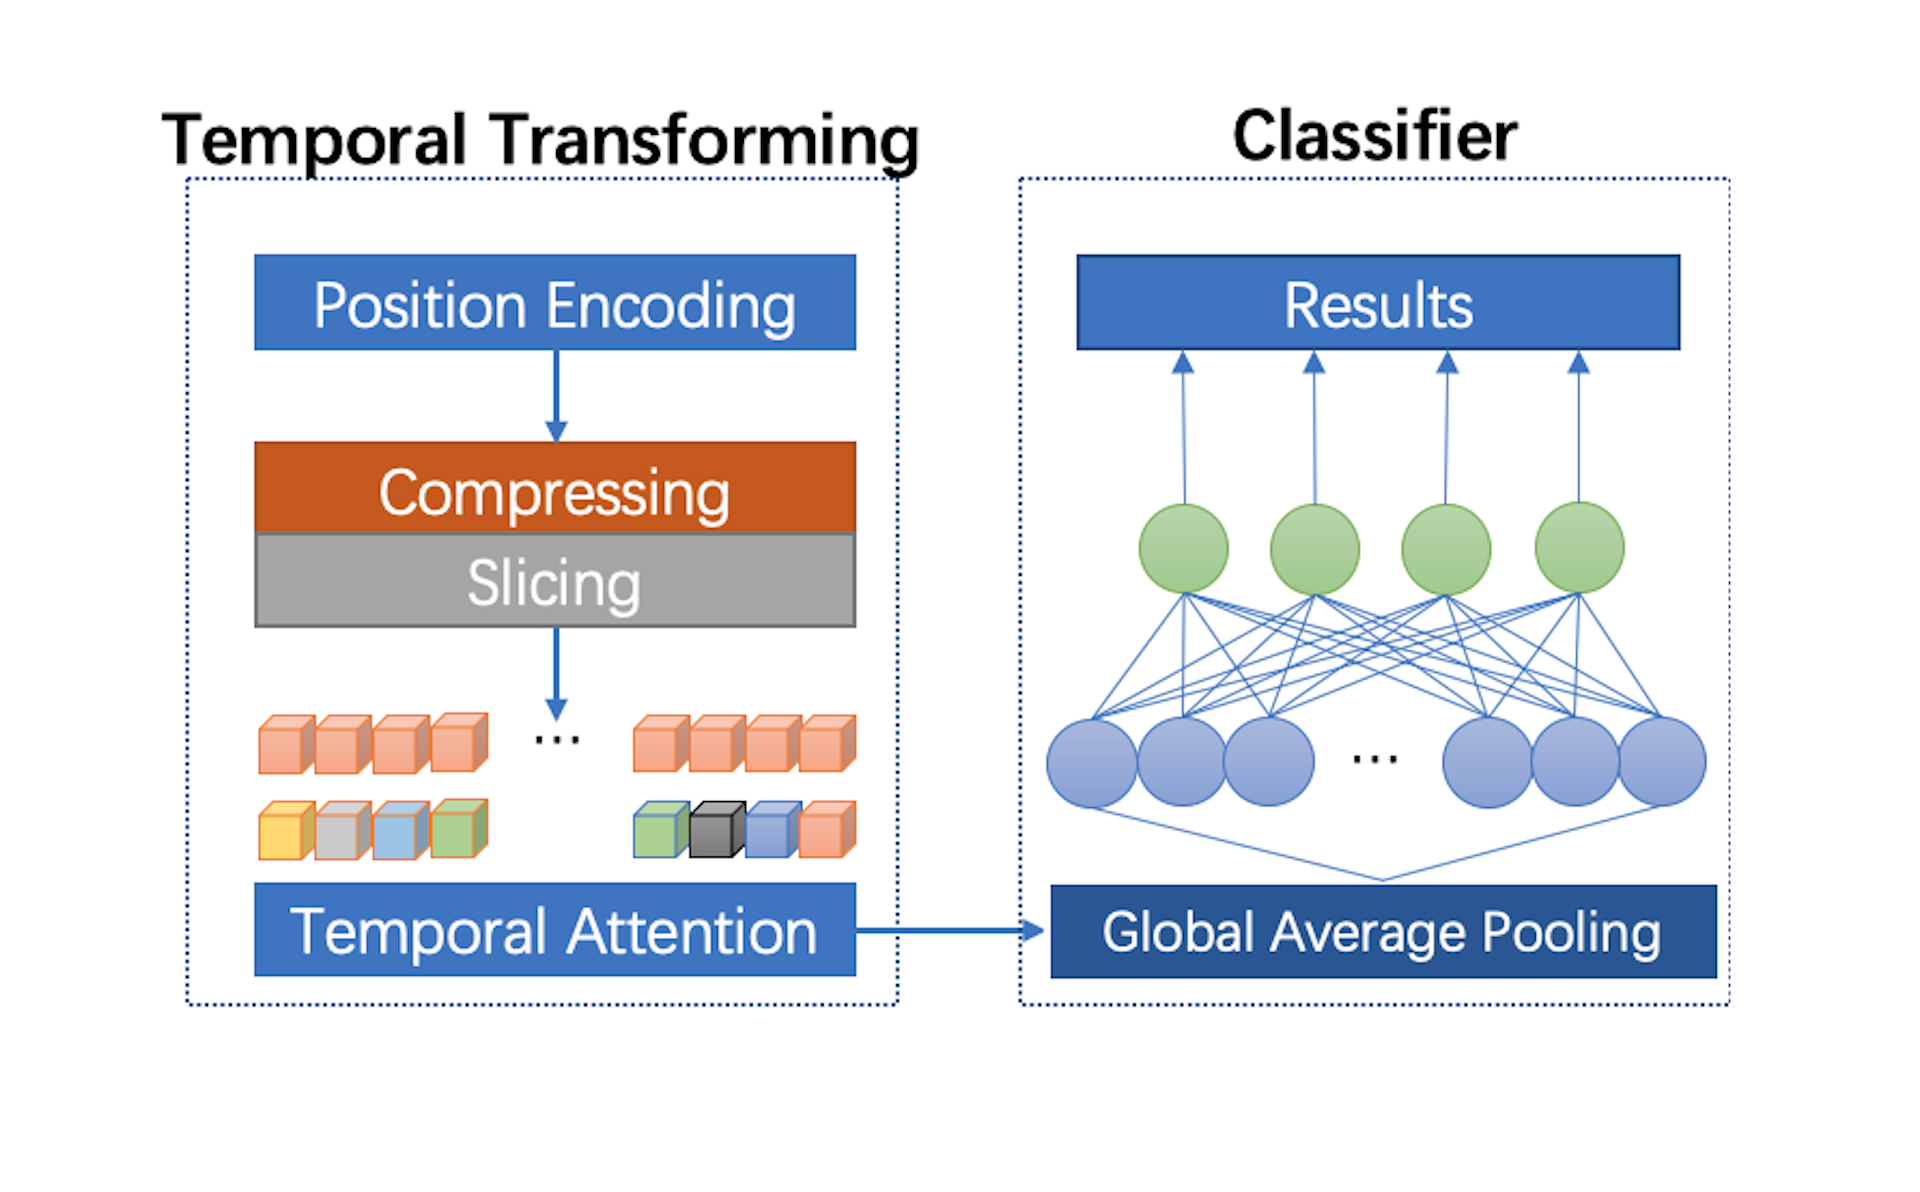
\includegraphics{figures/process}
\captionof{figure}{\color{Green}The overall frame of the Spatial-Temporal Transformer}
\label{process}
\end{center}
%----------------------------------------------------------------------------------------
%	RESULTS
%---------------------------------------------------------------------------------------- 
\color{Black}
\section*{Results}
We train this model under Google Colab environment with GPU Tesla T4. The slice size, $h$, $k_c$, and $N_f$ were 10, 5, 41, and 4. Additionally, in this model, we use Adam Optimizer with a learning rate of 0.0002. We also set our batch size to be 50, a dropout of 0.5 in temporal transforming and 0.3 in spatial transforming to avoid overfitting. Still, we compared the F1 score under different epoch while training, specific data are listed in Table 1.  F1 score can be calculated as $$F1\_score = 2(Recall * Precision) / (Recall + Precision)$$
\vspace{0.1cm}
\begin{center}
\captionof{table}{Epoch's influence on F1 score} 
\begin{tabular}{||c| c| c| c |c||} 
 \hline
 Epoch& Accuracy & Precision & Recall & F1-score\\ [1.5ex] 
 \hline\hline
 9 & 90.83 & 76.84 & 84.27 & 84.38 \\ 
 \hline
 10 & 91.94 & 83.75 & 80.14 & 82.91 \\
 \hline
 11 &91.61&86.78 & 81.18 & 85.94 \\
 \hline
 12 & 91.62 & 82.23 & 81.29 & 81.76 \\
 \hline
\end{tabular}
\end{center}
We can find the better result is always obtained by 11 epochs. Then to evaluate our model, we made comparative experiments with some other baselines. Brief descriptions are given as follows.
\begin{enumerate}
\item EEGNet$^8$, designs a compact and practical CNN with depthwise and separable convolutions to classify EEG.
\item CNN+LSTM$^9$, segments the original signal for OVR-CSP processing and extracts features with CNN, and the output is passed through an LSTM for temporal features.
\end{enumerate}
Through our investigation, we can conduct that under this scenario, our proposed model performs better.
\begin{center}
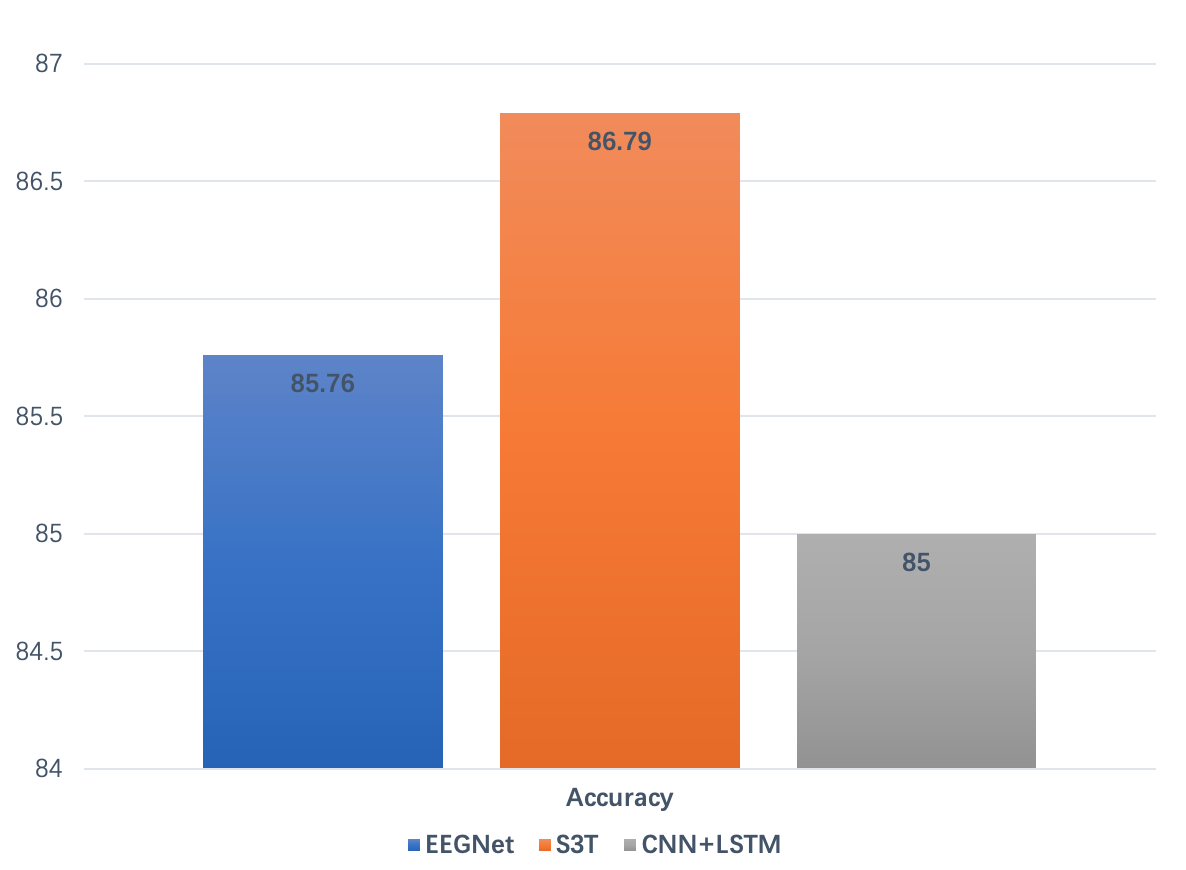
\includegraphics[width=0.7\linewidth]{figures/compare}
\captionof{figure}{\color{Green}The study results of 3 models}
\label{GIMlatlon}
\end{center}
%----------------------------------------------------------------------------------------
%	CONCLUSIONS
%----------------------------------------------------------------------------------------
\color{Black}
\section*{Summary}
At present, people usually use some convolutional neural network (CNN)-based methods for electroencephalogram (EEG) decoding. However, CNNs have limitations in perceiving global dependencies, which is insufficient for the common EEG paradigm with strong overall relationships. The EEG decoding method we proposed mainly relies on the attention mechanism. The EEG data is first preprocessed and spatially filtered. Then, we apply attention transformation on the feature channel dimension so that the model can enhance more relevant spatial features. \\
%The most critical step is to slice the data in the time dimension for attention conversion, and finally get a highly distinguishable representation. At this time, use global average pooling and a simple fully connected layer to classify different types of EEG data. 

Our model considers the spatial characteristics and timing of EEG signals on the basis of Convolutional Neural Network (CNN), and this is indeed an advantage of the proposed model.
Although this study is based on a limited number of EEG signals obtained from 53 subjects, the proposed algorithm achieves about 90\% accuracy rate and takes into account The spatial characteristics and timing of EEG signals. The proposed model can be used as a tool to objectively diagnose depression using EEG signals. In current clinical practice, the diagnosis of depression is based on questionnaire surveys and the patient's physical emotions. We hope this system can be used remotely by non-professional clinicians. Once the EEG signals are obtained from the patient, they will be sent to a server in the cloud (located in the hospital), where the proposed model can be used for diagnosis. The diagnosis result can be sent to the clinic immediately, as a reference for the diagnosis of professional clinicians.\\

%\hspace{0.1cm}$\circ$ text is derived from sections 1.10.33 of Cicero's De finibus bonorum et malorum;\\
%\hspace{0.1cm}$\circ$ text is derived from sections 1.10.33 of Cicero's De finibus bonorum et malorum;\\
%\hspace{0.1cm}$\circ$ text is derived from sections 1.10.33 of Cicero's De finibus bonorum et malorum;\\ 
%\hspace{0.1cm}$\circ$ text is derived from sections 1.10.33 of Cicero's De finibus bonorum et malorum;\\
%\hspace{0.1cm}$\circ$ text is derived from sections 1.10.33 of Cicero's De finibus bonorum et malorum;\\
%\hspace{0.1cm}$\circ$ text is derived from sections 1.10.33 of Cicero's De finibus bonorum et malorum;\\
%\hspace{0.1cm}$\circ$ text is derived from sections 1.10.33 of Cicero's De finibus bonorum et malorum.\\
%text is derived from sections 1.10.33 of Cicero's De finibus bonorum et malorumtext is derived from sections 1.10.33 of Cicero's De finibus bonorum et malorumtext is derived from sections 1.10.33 of Cicero's De finibus bonorum et malorumtext is derived from sections 1.10.33 of Cicero's De finibus bonorum et malorumtext is derived from sections 1.10.33 of Cicero's De finibus bonorum et malorumtext is derived from sections 1.10.33 of Cicero's De finibus bonorum et malorumtext is derived from sections 1.10.33 of Cicero's De finibus bonorum et malorumtext is derived from sections 1.10.33 of Cicero's De finibus bonorum et malorum.
%----------------------------------------------------------------------------------------
%	REFERENCE
%----------------------------------------------------------------------------------------
\section*{Reference}
\tiny \textnormal{1. Institute of Health Metrics and Evaluation. Global Health Data Exchange (GHDx).  http://ghdx.healthdata.org/gbd-results-tool?params=gbd-api-2019-permalink/d780dffbe8a381b25e1416884\\959e88b (Accessed 1 May 2021).}\\
\tiny \textnormal{2. A. Schwarz, M. K. Ho ̈ller, J. Pereira, P. Ofner, and G. R. Mu ̈ller-Putz, “Decoding hand movements from human EEG to control a robotic arm in a simulation environment,” Journal of Neural Engineering, vol. 17, no. 3, p. 036010, May 2020.}
\tiny \textnormal{3. A. Cruz, G. Pires, A. Lopes, C. Carona, and U. J. Nunes, “A Self-Paced BCI With a Collaborative Controller for Highly Reliable Wheelchair Driving: Experimental Tests With Physically Disabled Individuals,” IEEE Transactions on Human-Machine Systems, vol. 51, no. 2, pp. 109– 119, Apr. 2021.}\\
 \tiny \textnormal{4.Evans-Lacko S, Aguilar-Gaxiola S, Al-Hamzawi A, et al. Socio-economic variations in the mental health treatment gap for people with anxiety, mood, and substance use disorders: results from the WHO World Mental Health (WMH) surveys. Psychol Med. 2018;48(9):1560-1571. }\\
 \tiny \textnormal{5. Lee, M.H., Kim, N., Yoo, J. et al. Multitask fMRI and machine learning approach improve prediction of differential brain activity pattern in patients with insomnia disorder. Sci Rep 11, 9402 (2021). https://doi.org/10.1038/s41598-021-88845-w}\\
 \tiny \textnormal{6. Cai, H., Gao, Y., Sun, S., Li, N., Tian, F., Xiao, H., Li, J., Yang, Z., Li, X., Zhao, Q., Liu, Z., Yao, Z., Yang, M., Peng, H., Zhu, J., Zhang, X., Hu, X., \& Hu, B. (2020). MODMA dataset: a Multi-modal Open Dataset for Mental-disorder Analysis. arXiv preprint arXiv:2002.09283 }\\
 \tiny \textnormal{7. Song Y, Jia X, Yang L, et al. Transformer-based Spatial-Temporal Feature Learning for EEG Decoding[J]. arXiv preprint arXiv:2106.11170, 2021.}\\
 \tiny \textnormal{8. V.J.Lawhern,A.J.Solon,N.R.Waytowich,S.M.Gordon,C.P.Hung, and B. J. Lance, “EEGNet: a compact convolutional neural network for EEG-based brain–computer interfaces,” Journal of Neural Engineering, vol. 15, no. 5, p. 056013, Oct. 2018.}\\
 \tiny \textnormal{9. M. Lin, Q. Chen, and S. Yan, “Network In Network,” arXiv:1312.4400 [cs], Mar. 2014, arXiv: 1312.4400. [Online]. Available: http://arxiv.org/ abs/1312.4400}
\end{multicols}
%\textcolor{Orange}{\rule{\linewidth}{15pt}}
\vspace{0.5cm}
\end{framed}
\end{minipage}
%\hspace*{0.1cm}
\end{document}
%----------------------------------------------------------------------------------------
%%%%%%%%%%%%%%%%%%%%%%%%%%%%%%%%%%%%%%%%%%%%%%%%%%